\chapter{基于预训练辅助模型的Token表征学习}
\label{chap:Token}
本章主要对本文提出的基于预训练辅助模型的Token表征学习方法进行详细介绍,首先介绍其研究动机,接着阐述其方法设计,以及具体的实现过程,最后介绍实验验证过程和结果。

\section{研究动机}
\label{sec:TokenMotivation}

基于Token的代码表征方法本质上就是将源代码转换为一系列词法单元Token组成的序列,并对Token序列进行代码分析。

类似于自然语言技术处理文本,由于源代码中存在大量用户自己定义的标识符,不同用户的命名习惯不同,在对源代码的词法单元建模时,会产生一个规模巨大且稀疏的词汇表。该词汇表的规模会直接影响后续代码分析任务的效率,因此现有方法大多都对Token进行规范化,比如将变量名用统一的标识符来代替,从而降低词汇表的规模。但是后续神经网络模型训练过程中,当某个词汇在词汇表中没有出现过,那么神经网络模型就无法对其建模,即出现了在词汇表中不存在的Token,即集外词(Out-of-vocabulary,简称OOV)问题。有研究\cite{RJXB202205011}发现,针对代码表征中的集外词问题,在经典BigcloneBench\cite{7332459}数据集中OOV比率高达62.68\%,在OJClone数据集\cite{WOS:000485474201046}中OOV比率达到了16.82\%。

为了解决OOV问题,可以使用预训练模型增加词汇表的大小。近期,研究人员在大规模语料库上预训练各种语言模型,在解决各种自然语言处理任务方面取得了良好进展\cite{zhao2023survey}。在表征学习领域,也有基于大规模预训练模型提升代码表征能力的方法被提出。InferCode\cite{9402028}将自然语言处理中的自监督学习思想引入到代码的抽象语法树的表示中, 通过预测从AST上下文中自动识别的子树来训练代码表征,并且使用AST的子树作为训练标签,从而无需任何人工标记工作。该预训练InferCode模型可以应用于下游的无监督学习,例如代码聚类、代码克隆检测、跨语言代码搜索等。GraphCodeBERT\cite{guo2021graphcodebert}方法提出了一个基于数据流的代码表征预训练模型,与抽象语法树不同,数据流包含代码变量间“值从哪里来”的语义特征,并不会带来深层次不必要的复杂信息,使用该特征可以更有效的生成代码表征。然而这些预训练模型通常存在参数规模庞大, 训练及使用代价大的问题。

针对集外词OOV问题,本文提出一种基于预训练辅助模型的Token表征学习方法。通过从代码语料库中学习基本单元的语法语义信息,不断更新词汇表,扩大词汇表规模,从而减少出现集外词问题的概率。

\section{Token表征方法设计}
\label{sec:Token}
本节将主要介绍基于预训练辅助模型的Token表征学习方法的详细设计,首先介绍该方法的整体框架,并分别从预训练辅助词嵌入、Token代码表征两方面介绍具体设计。

\subsection{框架概述}
\label{subsec:TokenOverview}
本文提出的基于预训练辅助模型的Token表征学习方法整体框架如图\ref{fig:tokenframework}所示。该框架的输入是代码片段对应的Token序列,输出是对应的属性特征向量,主要包括预训练辅助词嵌入、Token代码表征两个阶段。

\begin{figure}[H]
  \centering
  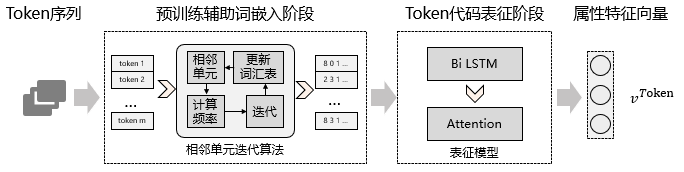
\includegraphics[width=0.95\textwidth]{figures/tokenframework}
  \caption{基于预训练辅助模型的Token表征学习框架}\label{fig:tokenframework}
\end{figure}

首先,预训练辅助词嵌入阶段以代码片段的Token序列作为训练数据,构建一个预训练辅助词嵌入模型。该模型的输入是代码片段对应的Token序列,输出为与输入对应的Token词嵌入向量。然后通过对模型的训练,使得该模型具有正确识别Token的能力,并将该模型保存下来。需要注意的是,为了减少集外词OOV问题,本文对模型采用相邻单元迭代算法,即,通过多次迭代来更新词汇表。

其次,Token代码表征阶段以Token词嵌入向量作为训练数据,构建一个Token表征模型。本文选用AttBiLSTM神经网络模型,该模型的输入是Token序列对应的词向量,输出为一个固定长度的密集向量用来表示代码的属性特征,主要包含两个部分:双向长短时记忆部分(BiLSTM)和自注意力机制部分(Attention),前者主要目的是同时捕获序列的双向语义信息,后者的主要目的是总结序列的输入特征,并将每个代码片段缩减为一个单一的密集向量。

在上述框架中,改进点主要体现在预训练辅助词嵌入阶段的相邻单元迭代算法、Token代码表征阶段的模型设计两方面。

\subsection{预训练辅助词嵌入阶段设计}
\label{subsec:TokenPreModel}

预训练辅助词嵌入阶段的主要目的是对于输入的词法单元Token序列进行词嵌入,生成的词汇表尽可能更多的词表单元,辅助后续表征阶段的嵌入,减少集外词问题出现的概率。因此,本文提出了一种相邻单元迭代算法(Adjacent token iterative algorithm,简称ATIA),该算法在词嵌入模型的基础上,通过组合Token序列中相邻单元构造新的代码表示单元,然后统计新单元出现的频率,根据频率信息多次迭代,不断更新词汇表,减少集外词问题。下面详细展开介绍预训练辅助阶段的具体设计。

首先,根据词嵌入模型生成基础词汇表。与自然语言处理类似,源代码的词法单元Token可以视为句子中的单词,Token维度的代码表征方法第一步就是将词法单元Token转换为机器易于理解和操作的数值向量,即词嵌入技术。它将词汇表中的每个单词转换成一个低维度、连续的向量表示,这种向量通常被称为词向量。目前,使用预训练词嵌入模型训练词向量的研究工作发展迅速,Word2vec、GloVe、FastText、ELMo和BERT等模型也相继被提出。其中,Word2vec模型通过从大规模无标注文本数据集中学习上下文信息,自动捕捉并编码词汇的语义关系,生成的词嵌入向量作为下游任务的输入特征,可以显著提升神经网络模型的性能和泛化能力。因此,本文采用Word2vec模型进行Token序列的词嵌入。

其次,依据相邻单元迭代算法更新词汇表。按照代码块组合相邻Token并查找出出现次数最频繁的Token组合,将这个组合称为新的迭代单元(Adjacent gram,简称Agram)。最后将这个Agram作为新的独立单元,加入到词汇表中,而原本组成这个Agram的原始Token单元并不会从词汇表中删除。在第一次迭代的时候,选取相邻的两两Token作为组合,把出现最频繁的Token组合确定为一个Agram单元之后再进行二次迭代,每次迭代在原来的基本单元上再组合一个新的邻近Token作为新的判断单元,不断的进行迭代,每次迭代都要对应的更新词汇表。

具体地,相邻单元迭代算法ATIA如算法\ref{alg1}所示。该算法有两个输入:待处理的初始Token语料库$Corpus$、迭代次数$N$,有两个输出:经过多次迭代后生成的语料库$NewCorpus$、词汇表$Vocab$,具体包括初始化AgramsSet、计算单元Agram出现的次数、更新语料库3个步骤,每个步骤的作用如下:

\begin{algorithm}[ht]  
	\renewcommand{\algorithmicrequire}{\textbf{Input:}}
	\renewcommand{\algorithmicensure}{\textbf{Output:}}
	\caption{Iterative algorithm}  
	\label{alg1}
	\begin{algorithmic}[1]
    \Require Origin Tokens Corpus:$Corpus$
    \Require The number of iterations:$N$
		\Ensure New Corpus: $New\_Corpus$
    \Ensure Vocabulary:$Vocab$
    \State $AgramsSet = \varnothing $ 
    \State $New\_Corpus \leftarrow Corpus $ 
    \State $Vocab = \left\{\right\} $  \Comment{step1:初始化}
		\For{$i \leftarrow 1$ to $N$}
      \If {i == 1}
        \For{token $in$ Corpus}
          \State add adjacent token to AgramsSet
        \EndFor 
      \Else
        \State numbers[] = \{\} 
        \For{Agram $in$ Aragms}
          \State Calculate the number of Argram in Corpus 
          \State add number to numbers \Comment{step2:计算单元Agram出现的次数} 
        \EndFor 
        \State $n \leftarrow $ Max(numbers) 
        \State $Max\_Agram \leftarrow$ Agram in Agrams whose number is n
        \State add $\left(Max\_Agram:n\right)$ to Vocab \Comment{step3:更新词汇表}
        \State add Agram to New\_Corpus \Comment{step3:更新语料库}
      \EndIf
    \EndFor \\
    \Return $New\_Corpus,Vocab$ 
	\end{algorithmic}
\end{algorithm}

(1)初始化:首先初始化一个AgramsSet用来存放Token组合(行1),初始化一个词汇表用来存放Token及其出现次数(行2),并且将目前已有的Token语料库$Corpus$添加进$NewCorpus$(行3)。

(2)计算单元Agram出现的次数:多次迭代,在第一次迭代时(行5-8),组合相邻Token,得到Agram组合,并添加进AragmsSet集合中。遍历语料库,计算AgramsSet中所有的Aragm出现的次数(行12),并且把Aragm组合当作key,组合出现的次数当作对应key的value值保存到词汇表(行13)。

(3)更新:遍历AragmsSet中所有的Agram的value值,将频率最高的Agram合并到新语料库中(行17-18)。然后重复(2)、(3)步骤,直到迭代次数N减少为0。

\subsection{Token代码表征阶段设计}
\label{subsec:TokenModel}

Token代码表征阶段的主要目的是根据上一阶段生成的辅助词汇表,构造一个Token表征模型,总结Token序列的整体特征,生成对应的属性特征向量。下面首先给出表征模型的选型,然后,基于该模型给出Token代码表征阶段的整体模型结构设计。

(1)模型选型

考虑到代码的Token序列是一种序列化的输入,并且前后词法单元可能存在依赖关系,为了更好地提高模型对Token序列数据的表征能力,本文选择双向长短期记忆网络BiLSTM模型来进行Token代码表征。

BiLSTM模型由一个正向的LSTM模型和一个反向的LSTM模型组成,主要思想是通过把序列向前、向后分别输入给两个独立的递归网络,这两个子网络连接到一个输出层,在每个词的输出部分把两个子网络的输出信息进行整合,这样网络就同时拥有了序列中每个词的过去时刻信息和未来时刻信息,更全面地捕捉序列信息,从而提高模型的性能。

\begin{figure}[htp]
  \centering
  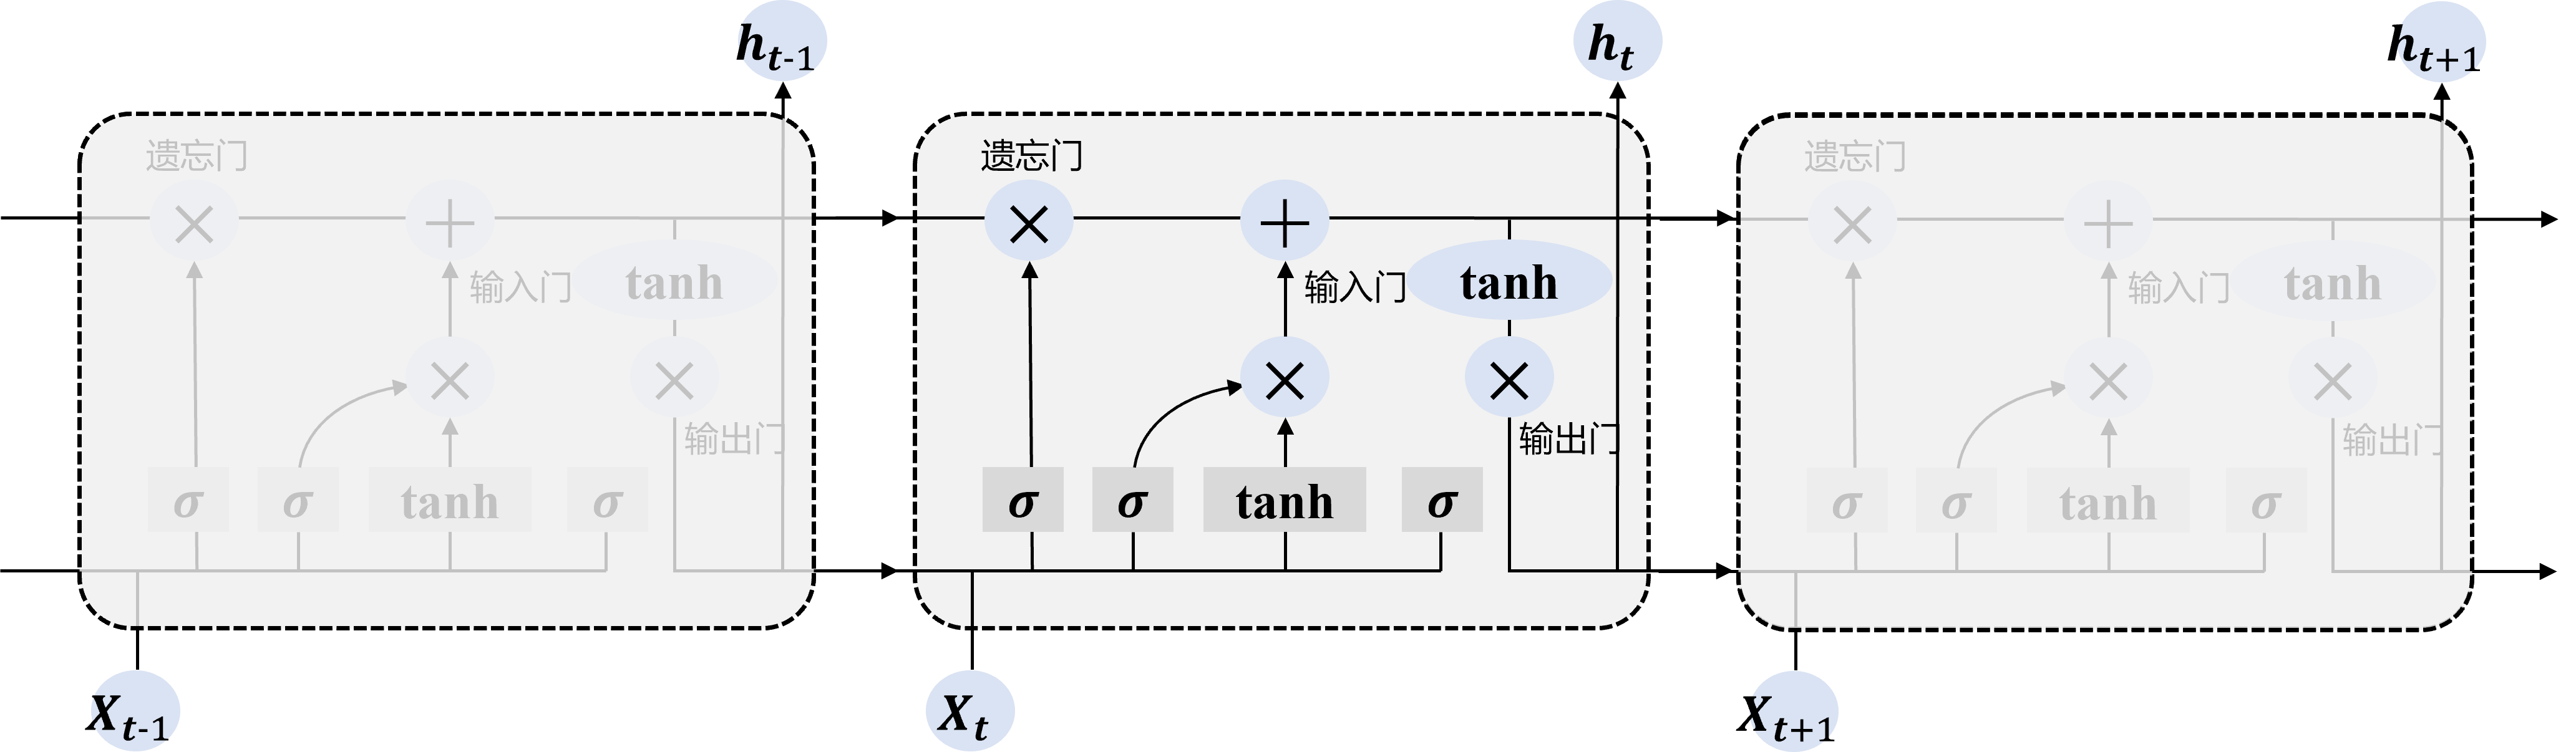
\includegraphics[width=0.8\textwidth]{figures/LSTM}
  \caption{LSTM模型时序结构图}\label{fig:LSTM}
\end{figure}

上图\ref{fig:LSTM}是长短期记忆网络LSTM的一个单元,每一个LSTM单元都有一个细胞状态和三个门(输入、输出、遗忘),通过三个门调节信息的流动,控制输入、自身状态、输出所占的比重,使网络能够在长时间内保留或遗忘信息。公式\ref{e3.1}-公式\ref{e3.6}给出了三个门控单元具体的计算方法。
\begin{equation}\label{e3.1}
  \begin{split}
    f_{t} = \sigma \left(W_{f} \cdot \left[h_{t-1},x_{t}\right] + b_f \right)
  \end{split}
\end{equation}
\begin{equation}\label{e3.2}
  \begin{split}
    i_t = \sigma \left(W_{i} \cdot \left[h_{t-1},x_{t}\right] + b_i\right)
  \end{split}
\end{equation}
\begin{equation}\label{e3.3}
  \begin{split}
    \widetilde{C_t} &= \tanh \left(W_{c} \cdot \left[h_{t-1},x_{t}\right] + b_c \right)
  \end{split}
\end{equation}
\begin{equation}\label{e3.4}
  \begin{split}
    C_t = f_t \otimes C_{t-1} + i_t \otimes \widetilde{C_t}
  \end{split}
\end{equation}
\begin{equation}\label{e3.5}
  \begin{split}
   out_t = \sigma \left(W_{out} \cdot \left[h_{t-1},x_{t}\right] + b_o \right)
  \end{split}
\end{equation}
\begin{equation}\label{e3.6}
  \begin{split}
   h_t = out_t \otimes \tanh \left(C_t\right)
  \end{split}
\end{equation}

其中,公式\ref{e3.1}表示遗忘门,用来决定在当前时间步的存储状态中传递前一个时间步的哪些信息。其中$h_{t-1}$表示上一个时间步的隐藏状态,$x_{t}$表示为当前时间步的输入数据,$\sigma$表示为非线性激活sigmoid函数,得出的值越接近0越有可能被丢弃,越接近1越有可能被记住;公式\ref{e3.3}表示输入门,用来确定输入的$x_{t}$中哪些信息能够传递到当前时间步,同时依赖于$tanh$ 和 $sigmoid$函数,得到当前时间步中需要记录的值$\widetilde{C_t}$;公式\ref{e3.5}表示输出门,用来确定当前时间步的信息有多少能够传递到下一个时间步,$C_t$表示为当前时刻细胞的最终状态,$f_{t}$来控制丢弃旧细胞信息,同时加上新的重要信息。最终输出长期状态$C_t$和短期记忆$h_t$。长期状态$C_t$从左到右经过LSTM单元,通过遗忘门丢失一些前时间步信息,通过输入门添加当前时间步信息,最后通过输出门输出。

LSTM模型存在一个问题,即无法获取从后往前的信息。因此在LSTM基础上,引入双向长短期记忆网络LSTM模型,从前后两个方向获取信息。

\begin{figure}[htp] 
  \centering
  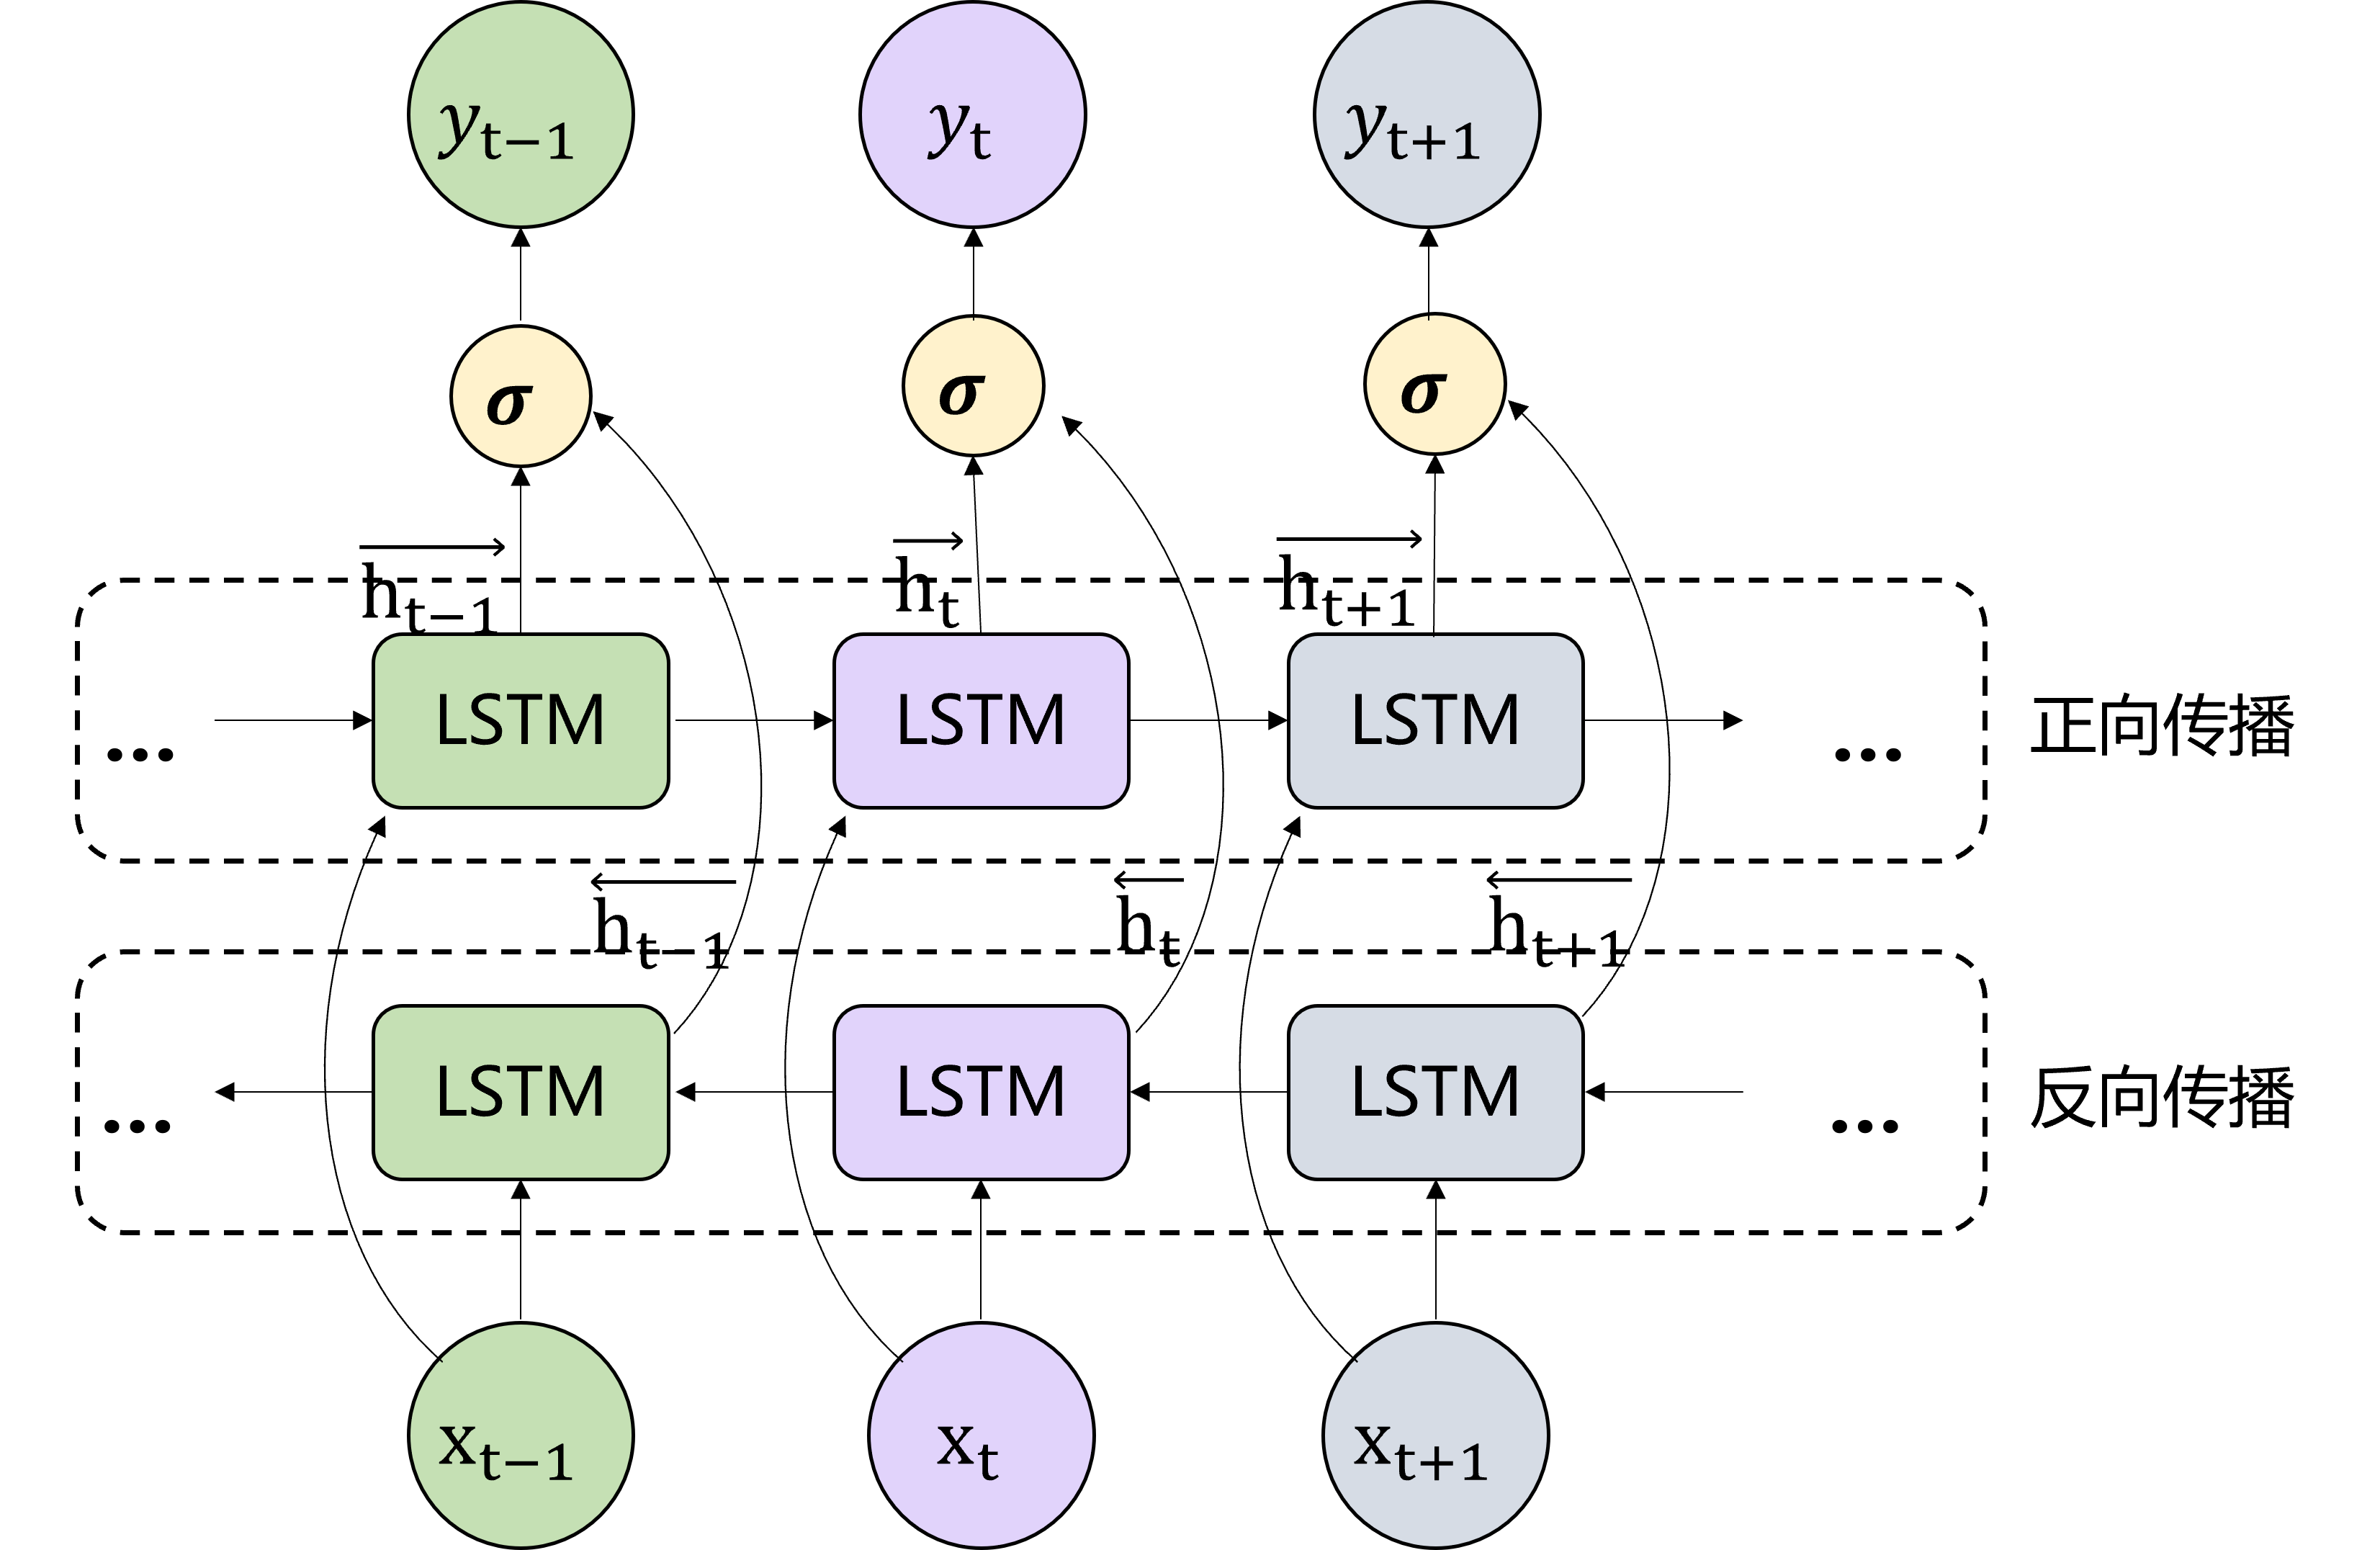
\includegraphics[width=0.5\textwidth]{figures/BiLSTM}
  \caption{BiLSTM模型结构}\label{fig:BiLSTM}
\end{figure}

上图\ref{fig:BiLSTM}是双向长短期记忆网络BiLSTM模型的结构,包含一个正向的LSTM层和一个反向的LSTM层。公式\ref{e3.7}-公式\ref{e3.8}给出了BiLSTM模型具体的计算方法。
\begin{equation}\label{e3.7}
  \begin{split}
    \overrightarrow{y_t} &= W_0 \cdot LSTM\left(x_{t},\overrightarrow{h_{t-1}}\right) + b_0
    \\
    \overleftarrow{y_t} &= W_0 \cdot LSTM\left(x_{t},\overleftarrow{h_{t-1}}\right) + b_0
  \end{split}
\end{equation}
\begin{equation}\label{e3.8}
  \begin{split}
    y_t = \overrightarrow{y_t} \oplus\overleftarrow{y_t}
  \end{split}
\end{equation}

其中,$\overrightarrow{h_t}$表示$t$时刻的前向隐藏状态,$\overrightarrow{h_t}$表示向后隐藏状态,$\overrightarrow{y_t}$表示向前输出,$\overleftarrow{y_t}$表示向后输出。公式\ref{e3.7}给出当前状态$\overrightarrow{y_t}$和$\overleftarrow{y_t}$的计算公式。公式\ref{e3.8}给出当前$t$时刻的最终输出$y_t$,它通过对当前状态$\overrightarrow{y_t}$和$\overleftarrow{y_t}$进行拼接得到。

(2)Token维度代码表征整体模型结构设计

基于BiLSTM模型,给出Token维度代码表征阶段整体模型结构设计,如图\ref{fig:tokenmodel}所示。该模型主要包括输入层、双向长短时记忆层(BiLSTM)和自注意力机制层(Attention)、输出层。
\begin{figure}[htp]
  \centering
  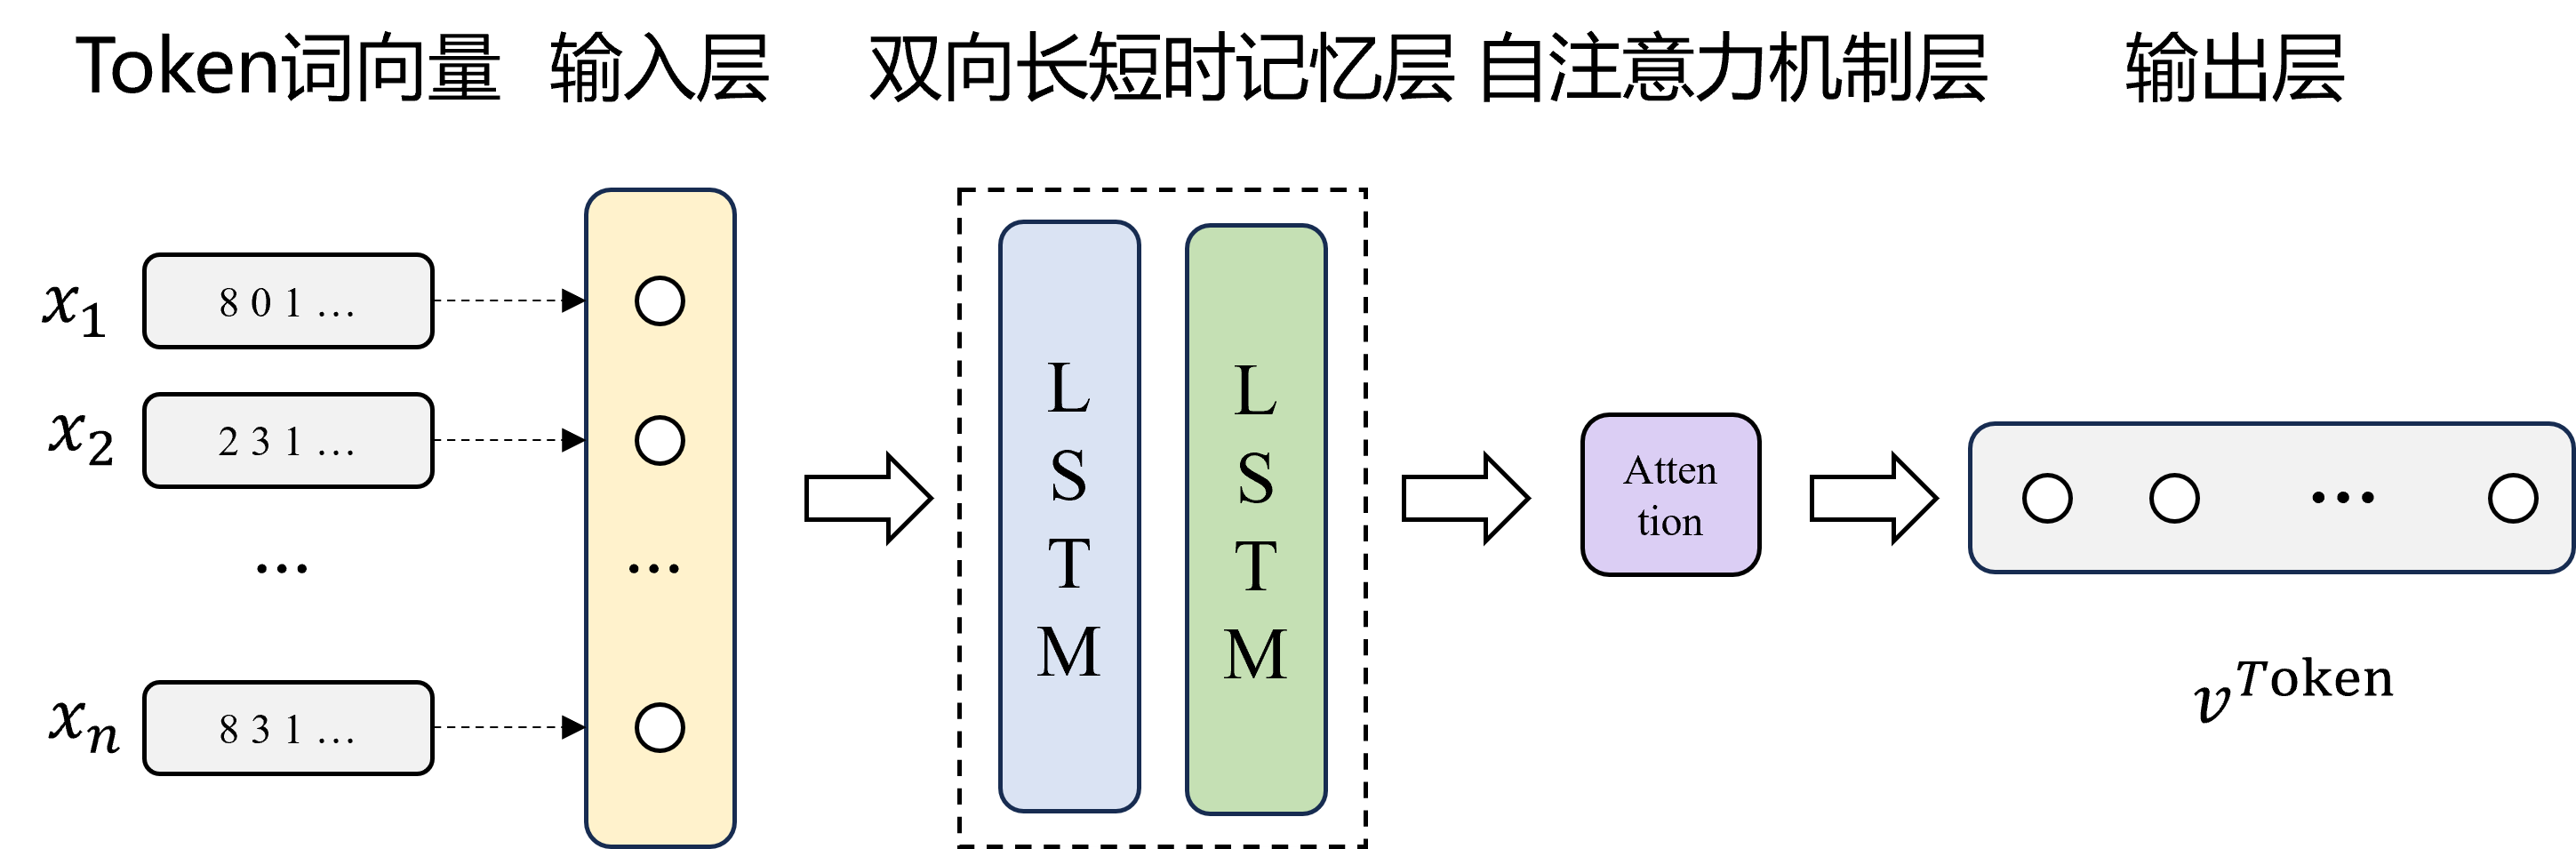
\includegraphics[width=0.5\textwidth]{figures/tokenmodel}
  \caption{Token维度代码表征模型AttBiLSTM结构}\label{fig:tokenmodel}
\end{figure}

\ding{172}输入层:输入层用于向模型输入训练数据,在本方法中模型的输入为经过预训练辅助嵌入模型得到的Token序列词向量,即每个词向量对应一个输入神经元。\ding{173}双向长短时记忆层:由两层LSTM构成,一个正向的LSTM层从前往后捕获Token序列语义信息,一个反向的LSTM层从后往前捕获Token序列语义信息。\ding{174}自注意力机制层:本层的主要目的是总结序列的输入特征,并将每个代码片段缩减为一个单一的密集向量。\ding{175}输出层:每个Token序列对应一个输出。

\section{Token表征方法示例}
\label{sec:Tokenachieve}

为了更形象地描述本文提出的基于预训练辅助模型的Token表征方法,本节给出一个示例。下图\ref{fig:code}是三个简单的代码片段,其主要功能为计算数组元素之和。

\begin{figure}[htp] 
  \centering  %居中
  \subfigure[C语言代码片段1]{   %第一张子图
      \centering    %子图居中
      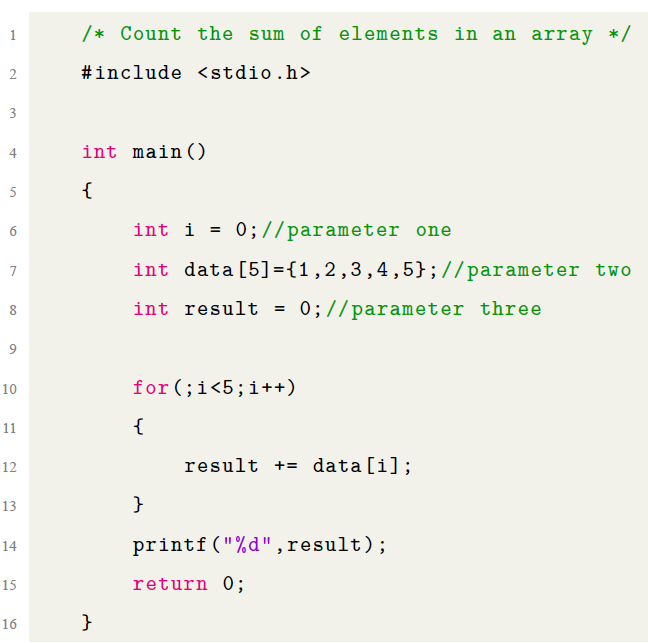
\includegraphics[width=0.3\textwidth]{figures/code1}
      \label{fig:code1} %引用标签
  }
  \subfigure[C语言代码片段2]{ %第二张子图
      \centering    %子图居中
      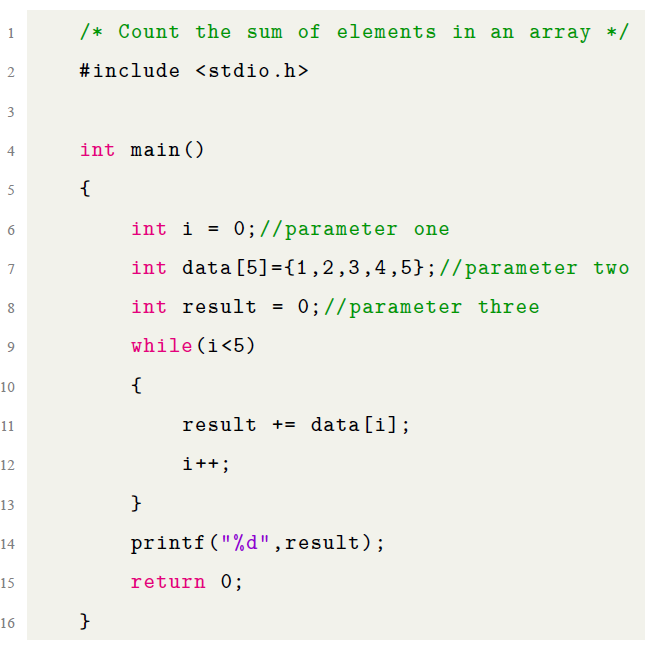
\includegraphics[width=0.3\textwidth]{figures/code2}
      \label{fig:code2} %引用标签
  }
  \subfigure[C语言代码片段3]{ %第三张子图
      \centering    %子图居中
      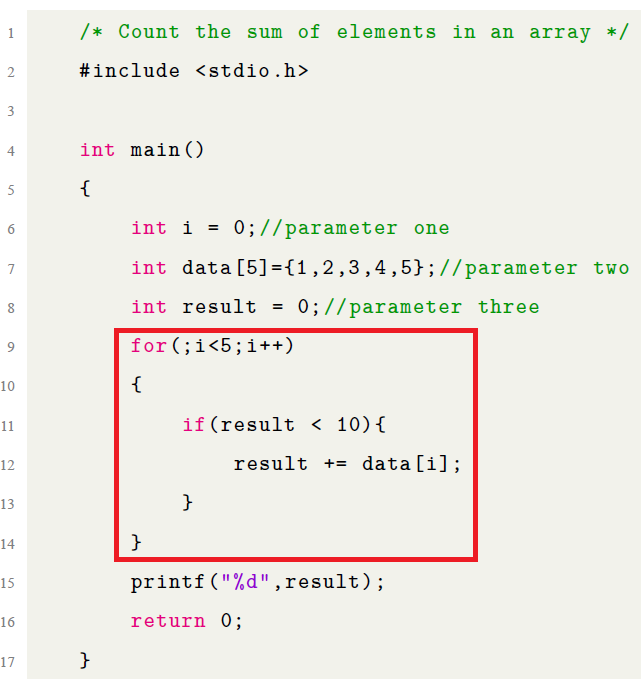
\includegraphics[width=0.3\textwidth]{figures/code3}
      \label{fig:code3} %引用标签
  }
  \caption{C语言代码片段示例}    %大图名称
  \label{fig:code}    %图片引用标记
\end{figure}

其中图\ref{fig:code1}的第10-13行采用for循环,图\ref{fig:code2}的第9-13行采用while循环,这两个代码片段属于真克隆对;图\ref{fig:code2}的第9-14行采用for循环,但在内部需要判断result的现有状态,因此图\ref{fig:code1}和图\ref{fig:code3}的代码片段属于假克隆对。

经过\ref{subsec:Preprocess}小节的代码预处理阶段,可以得到对应的Token序列,如图\ref{fig:token}。分析红框内的Token可以发现,真克隆对的Token序列只有一个词不同,而假克隆对的Token序列中不同的词法单元数目很多。

\begin{figure}[htp] 
  \centering  %居中
  \subfigure[代码片段1对应的Token序列]{   %第一张子图
      \centering    %子图居中
      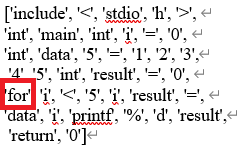
\includegraphics[width=0.3\textwidth]{figures/token1}
      \label{fig:token1} %引用标签
  }
  \subfigure[代码片段2对应的Token序列]{ %第二张子图
      \centering    %子图居中
      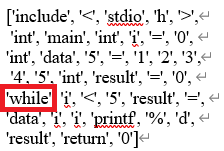
\includegraphics[width=0.3\textwidth]{figures/token2}
      \label{fig:token2} %引用标签
  }
  \subfigure[代码片段3对应的Token序列]{ %第三张子图
      \centering    %子图居中
      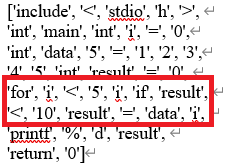
\includegraphics[width=0.3\textwidth]{figures/token3}
      \label{fig:token3} %引用标签
  }
  \caption{代码片段示例对应的Token序列}    %大图名称
  \label{fig:token}    %图片引用标记
\end{figure}
% \lstset{language=C}
% \begin{lstlisting}
%     /* Count the sum of elements in an array */
%     #include <stdio.h>
    
%     int main()
%     {
%         int i = 0;//parameter one
%         int data[5]={1,2,3,4,5};//parameter two
%         int result = 0;//parameter three
        
%         for(;i<5;i++)
%         {
%             result += data[i];
%         }
%         printf("%d",result); 
%         return 0;
%     }
% \end{lstlisting}

% \lstset{language=C}
% \begin{lstlisting}
%     /* Count the sum of elements in an array */
%     #include <stdio.h>
    
%     int main()
%     {
%         int i = 0;//parameter one
%         int data[5]={1,2,3,4,5};//parameter two
%         int result = 0;//parameter three
%         while(i<5)
%         {
%             result += data[i];
%             i++;
%         }
%         printf("%d",result); 
%         return 0;
%     }
    
% \end{lstlisting}

% \lstset{language=C}
% \begin{lstlisting}
%     /* Count the sum of elements in an array */
%     #include <stdio.h>
    
%     int main()
%     {
%         int i = 0;//parameter one
%         int data[5]={1,2,3,4,5};//parameter two
%         int result = 0;//parameter three
%         for(;i<5;i++)
%         {
%             if(result < 10){
%                 result += data[i];
%             }
%         }
%         printf("%d",result); 
%         return 0;
%     }
% \end{lstlisting}

本章提出的基于预训练辅助模型的Token表征学习方法对代码片段示例的处理流程如图\ref{fig:token}所示。基于上述示例,自底向上,该方法的输入是一对代码片段$C_{a},C_{b}$对应的Token序列,表示为$\left( w_{1}^{a},w_{2}^{a},\ldots,w_{m}^{a}\right)$ 和 $\left( w_{1}^{b},w_{2}^{b},\ldots,w_{n}^{b} \right)$,输出是$C_{a},C_{b}$对应的属性特征向量 $V_{a}^{Token},V_{b}^{Token}$,整体采用Siamese架构,两个子网络共享权值,从下到上,主要包括预训练辅助词嵌入、Token代码表征两个阶段。
\begin{figure}[htp]
  \centering
  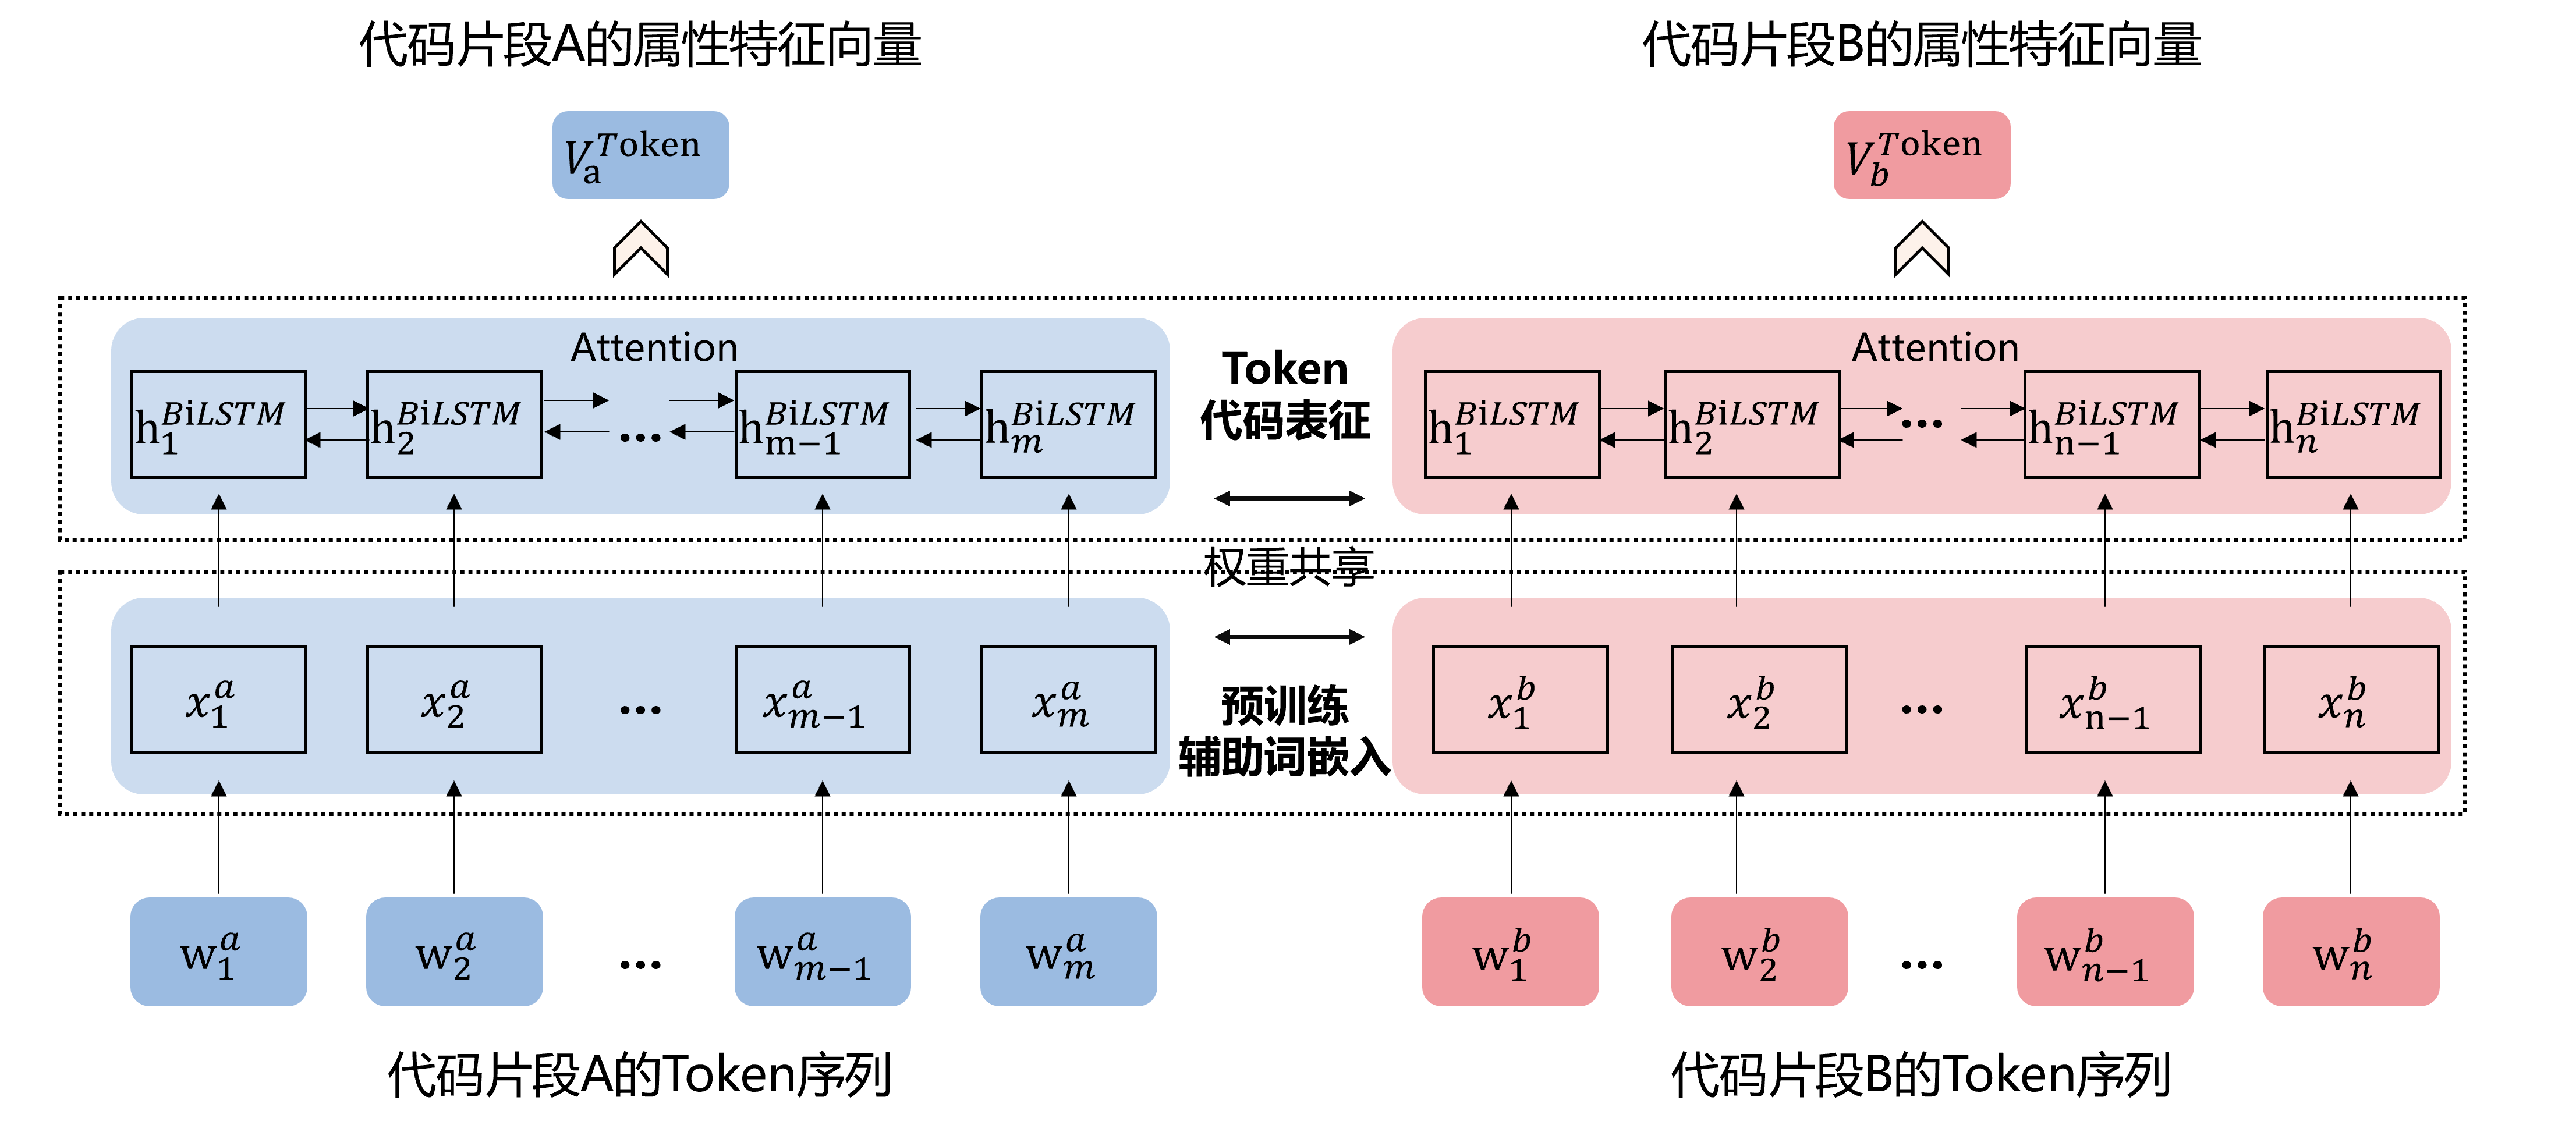
\includegraphics[width=0.9\textwidth]{figures/token}
  \caption{基于预训练辅助模型的Token表征学习方法示例}\label{fig:token}
\end{figure}

具体来说,在预训练辅助词嵌入阶段,对于代码片段$C_{a}$,经过分割得到的Token序列$\left( w_{1}^{a},w_{2}^{a},\ldots,w_{m}^{a}\right)$,($m$是代码片段A的长度),然后在词汇表$E_{w}$中查找每个Token对应的向量,将所有的token $w_{i}^{a} \left(i \in [1,m]\right)$ 转化为密集向量。其中查找词汇表$E_{w}$已经经过代码语料库使用相邻单元迭代算法ATIA基于Word2vec模型进行预训练,在模型中是固定的。其查找过程可以表示为公式\ref{e3.9}:

\begin{equation}\label{e3.9}
  \begin{split}
  x_{i}^{a} = lookup\_Token \left(w_{i}^{a} ,E_{w} \right)
  \end{split}
\end{equation}

经过嵌入阶段的预训练后,代码片段$C_{a}$生成了序列$\left( x_{1}^{a},x_{2}^{a},\ldots,x_{m}^{a}\right)$。使用同样的嵌入方式,可以得到对于Token序列$\left( w_{1}^{b},w_{2}^{b},\ldots,w_{n}^{b}\right)$,($n$是代码片段B的长度)的向量表示$\left( x_{1}^{b},x_{2}^{b},\ldots,x_{n}^{b} \right)$。

在Token代码表征阶段,将代码向量的Token序列作为输入,使用BiLSTM模型进行编码。处理过程分为两个步骤,如公式\ref{e3.10}所示:

\begin{equation}\label{e3.10}
  \begin{split}
    h_{1}^{aBiLSTM},h_{2}^{aBiLSTM},\ldots,h_{n}^{aBiLSTM} = BiLSTM \left(x_{1}^{a},x_{2}^{a},\ldots,x_{m}^{a}\right) \\
    V_{a}^{Token} = Attention \left( h_{1}^{aBiLSTM},h_{2}^{aBiLSTM},\ldots,h_{n}^{aBiLSTM} \right)
  \end{split}
\end{equation}

经过嵌入阶段的预训练后,每一个Token $w_{i}^{a}$ 都被转换为一个密集向量$x_{i}^{a}$,经过BiLSTM编码后,生成了$h_{i}^{aBiLSTM}$,然后经过Attention层的总结后,生成了$V_{a}^{Token}$作为代码片段$C_{a}$的最终Token表示,即属性特征向量。
同样,可以使用相同的计算以$\left( x_{1}^{b},x_{2}^{b},\ldots,x_{n}^{b} \right)$作为输入为代码片段$C_{b}$计算$V_{b}^{Token}$。

\section{实验验证}
\label{sec:TokenExperiment}
为了验证基于预训练辅助模型的Token表征方法的有效性,本节展开实验验证。首先,介绍了实验整体的环境配置、数据集,以及实验评估指标;接着,对基于预训练模型的Token表征方法进行了消融实验,探究本章创新点:预训练辅助模型使用的语料库规模、Token表征模型对代码克隆检测任务实验结果的影响。

\subsection{实验环境}
\label{subsec:Environment}
本章的实验验证均运行于Linux系统下,实验对于软硬件环境有一定的要求,在硬件方面需要一定的显卡来提升模型训练速度,软件方面需要代码分析工具Joern生成对应的抽象语法树、程序依赖图,并依赖深度学习库来实现模型,具体的系统配置如表\ref{tab:environment}所示。
\begin{table}[htp]
  \centering
  \caption{实验环境配置} 
  \label{tab:environment}
  \renewcommand{\arraystretch}{1.1}
  \begin{tabular*}{0.5\textwidth}{@{\extracolsep{\fill}}cc}
  \toprule
    环境			&配置		\\
  \midrule
    操作系统		&Ubuntu 20.04 \\
    处理器			&Intel Core i9-12900KF × 24 \\
    内存			  &31.1G \\
    显卡			  &NVIDIA  \\
    磁盘			  &1TB \\
    开发语言    &Python3.6 \\
    主要工具和框架 &Joern、Pytorch1.10 \\
  \bottomrule
  \end{tabular*}
\end{table}

\subsection{实验数据集构建}
\label{subsec:Dataset}
本章实验是为了验证预训练辅助模型在Token层面上表征学习的有效性,因此在数据集的选取上,本文针对C语言选取了POJ104数据集。如表\ref{tab:dataset}所示。POJ104数据集是一个基于C语言所构建的大型数据集。OJ系统是一个以编程教学为目的的公开评判系统,共存在104个编程问题,针对每个编程问题,学生们通过在线提交自己的代码来尝试解决,同时OJ系统将自动判断提交源代码的正确性和有效性。对于OJ系统来说,同一个问题的不同答案可以看作一对真克隆对,不同问题的答案可以视为一对假克隆对。POJ104数据集针对每一个编程问题,均提供500个学生提交的源代码,即共有52000个样本。

\begin{table}[htp]
  \centering
  \caption{POJ104数据集} 
  \label{tab:dataset}
  \renewcommand{\arraystretch}{1.1}
  \begin{tabular*}{0.5\textwidth}{@{\extracolsep{\fill}}cc}
  \toprule
    名称			&统计信息		\\
  \midrule
    Dataset			&POJ104数据集 \\
    Language    &C \\
    Program			&52000 \\
    Classes			&104 \\
    Max tokens			&8737 \\
    Avg tokens			&245 \\
  \bottomrule
  \end{tabular*}
\end{table}

(1) 数据集预处理

首先对数据集进行初步筛选,去掉其中包含乱码的样本,共得到51485个源代码样本。然后对源代码进行预处理,通过深入研究并比较现有标记转换规则,发现CCLearner\cite{10.1145/1287624.1287634}对转换规则进行了实验评估,验证各个标记的有效性,因此本文参考CCLearner\cite{10.1145/1287624.1287634}这篇文献的转换规则,对标识符进行了归一化处理。具体地,保留if、for等关键词,数字常量值用NUM替代,字符串用String替代等。删除样本中包含的空白行和注释等多余代码,并将数据集保存到一个program.pkl文件中,program.pkl文件中一共包含51485行×3列的数据集,每一行数据代表一个源代码样本,第一列为源代码id,第二列保存源代码样本code,第三列为源代码的标签label,即属于哪一个编程问题。

(2) 构造代码克隆对

本文随机两两组合同一标签label的源代码,组成5200个真克隆对,随机组合不同标签的源代码组成44800个假克隆对,一共包含50000个克隆对,并将其保存到oj\_clone\_ids.pkl文件中,oj\_clone\_ids.pkl文件中一共包含50000行×3列的数据集,每一行数据代表一个克隆对样本,第一列为源代码id1,第二列为源代码id2,第三列为克隆对的标签label,真克隆对标签为1,假克隆对标签为0。最后,依据随机种子将数据集按照3:1:1划分为训练集、测试集、验证集,其中的正负样本数如下表\ref{tab:ClonePairs}所示。

\begin{table}[htp]
  \centering
  \caption{本文预处理后的POJ104数据集正负样本数} 
  \label{tab:ClonePairs}
  \renewcommand{\arraystretch}{1.1}
  \begin{tabular*}{0.8\textwidth}{@{\extracolsep{\fill}}cccc}
  \toprule
    数据集			&真克隆对		&假克隆对		&克隆对数 \\
  \midrule
    训练集train			&3162	  &26838		&30000 \\
    测试集test			&1022		&8978		  &10000 \\
    验证集dev			  &1016		&8984		  &10000 \\
    总计            &5200	  &44800	  &50000 \\
  \bottomrule
  \end{tabular*}
\end{table}

\subsection{评估指标}
\label{subsec:Index}
代码克隆检测问题是二分类问题,因此本文采用精确率(Precision)、召回率(Recall)、F1值三个评估指标来度量实验结果,其中使用了混淆矩阵中的真阳性(True Positive, TP)、假阳性(False Positive, FP)、假阴性(False Negative, FN)、真阴性(True Negative, TN),如表\ref{tab:ConfusionMatrix}所示。

\begin{table}[htp]
  \centering
  \caption{分类问题的混淆矩阵} 
  \label{tab:ConfusionMatrix}
  \renewcommand{\arraystretch}{1.1}
  \begin{tabular*}{0.7\textwidth}{@{\extracolsep{\fill}}ccc}
  \toprule
  \multirow{2}{*}{实际值} & \multicolumn{2}{c}{预测值} \\
  \cmidrule{2-3} 
  \multirow{2}{*}{} & 正样本(P) & 负样本(N) \\
  \midrule
    正样本(P)			&TP	  &FN		 \\
    负样本(N)			&FP		&TN		 \\
  \bottomrule
  \end{tabular*}
\end{table}

其中,混淆矩阵中的真阳性TP表示样本实际为正样本,并且被模型预测为正样本,即实际上标记为真克隆对并且被检测出来为真克隆对的代码对;假阳性FP表示样本实际为负样本,但是被模型预测为正样本,即实际上标记为假克隆对但是被检测出来为真克隆对的代码对;假阴性FN表示样本实际为正样本,但是被模型预测为负样本,即实际上标记为真克隆对但是被检测出来为假克隆对的代码对;真阴性TN表示样本实际为负样本,并且被模型预测为负样本,即实际上标记为假克隆对并且被检测出来为假克隆对的代码对。

因此,本文采用的评估指标如公式\ref{e3.11}-公式\ref{e3.13}所示。
\begin{equation}\label{e3.11}
  Precision = \frac{TP}{TP+FP} 
\end{equation}
\begin{equation}\label{e3.12}
  Recall = \frac{TP}{TP+FN} 
\end{equation}
\begin{equation}\label{e3.13}
  F1 = \frac{2*Precision*Recall}{Precision+Recall} 
\end{equation}

其中,精确率(Precision)表示正确检测到的代码克隆数量占全部预测为代码克隆的比例;召回率(Recall)表示正确检测到的代码克隆数量占总体实际代码克隆数量的比例;精确率(Precision)和召回率(Recall)指标有时候会出现的矛盾时,综合考虑两者的表现,使用F1值用于评价分类模型的好坏。

\subsection{预训练语料库规模实验结果}
\label{subsec:TokenResult1}

本节实验的目的是评估改进点1:预训练辅助模型中使用的预训练语料库规模是否可以减少集外词问题出现的概率,提升Token维度的代码表征能力?

具体地,在\ref{subsec:Dataset}节构造的数据库中随机选取了100对、200对、500对代码克隆对作为预训练数据集,构造预训练语料库,基于相邻单元迭代算法开展预训练,计算辅助词汇表长度,通过分析下游代码克隆检测任务的准确率判断Token维度代码表征能力。本文在实验中采用单一变量原则,仅修改了预训练数据库规模,后续Token表征模型均采用AttBiLSTM模型。具体实验结果如表\ref{tab:category}所示。

\begin{table}[htbp]
  \centering  
  \caption{预训练辅助模型使用的语料库规模对实验结果的影响}   
  \label{tab:category}  
  %\renewcommand{\arraystretch}{1.1}
  \begin{tabular*}{0.9\textwidth}{@{\extracolsep{\fill}}ccccc}  
  \toprule
  \multirow{2}{*}{预训练数据集规模} & \multirow{2}{*}{词汇表长度} & \multicolumn{3}{c}{POJ104} \\
  \cmidrule{3-5} 
   & & 准确率P(\%) & 召回率R(\%) & F1值(\%)  \\  
  \midrule 
  100对	&240		& 89.74	& 87.84	& 88.78		 \\  
  300对	&463		& 89.76	& 90.24	& 90.00	 \\  
  500对	&593 	  & 89.78	& 95.62	& 92.61	   \\  
  \bottomrule  
  \end{tabular*}  
\end{table}

基于对表\ref{tab:category}数据的分析,可以看出:(1)随着预训练语料库的增大,Word2vec模型预训练的词表长度也不断增大。当数据集规模增加5倍的同时,词表长度也增加了2倍多。(2)随着预训练词表长度的增加,代码克隆检测任务的F1值呈现上升趋势,即对代码克隆的检测效果会不断增强。当预训练数据库规模达到500对时,其F1值上涨至92.61\%,说明通过预训练得到的词汇表每个词的向量表示可以很好的表征这个词的代码信息。

通过上述分析得到结论:本文提出的预训练辅助模型生成的辅助词汇表长度增加,集外词问题出现的概率下降,对应生成的词嵌入向量作为下游任务的输入特征,可以提升下游神经网络模型的检测能力。考虑到需要预留出足够的答案样本用来构造训练集和测试集,最终选择500对源代码作为C语言实验中的预训练数据集大小。

\subsection{Token表征模型实验结果}
\label{subsec:TokenResult2}

本节实验的目的是评估改进点2:Token表征模型的选取是否影响Token维度的代码表征能力?具体地,将AttBiLSTM模型与双向RNN、LSTM与BiLSTM模型进行对比,同时本文在实验中采用单一变量原则,预训练辅助模型采用500对预训练数据集生成,RNN、LSTM、BiLSTM模型均基于Pytorch1.10实现,其参数设置如表\ref{tab:parameter}所示。参数的确定是通过多次调试后选择最优参数作为最后的结果。Token表征模型实验结果如下表\ref{tab:category2}所示。

\begin{table}[htbp] 
  \centering  
  \caption{模型参数设置}   
  \label{tab:parameter}  
  %\renewcommand{\arraystretch}{1.1}
  \begin{tabular*}{0.9\textwidth}{@{\extracolsep{\fill}}ccc}  
  \toprule  
  参数 & 类别 & 具体参数  \\  
  \midrule
  \multirow{3}{*}{预训练辅助模型} & 词嵌入层维度	& 128		 \\  
  & 词汇表大小	& 593		\\
  & 代码序列长度	& 500		\\  
  \cmidrule{2-3} 
  \multirow{8}{*}{Token表征模型}   & LSTM层数	& 2		 \\  
  & 损失函数Loss	& BCELoss		\\
  & 优化器Optimizer	& Adam		\\  
  & 学习率lr	& 0.001		 \\  
  & 丢弃概率Dropout	& 0.5		\\
  & 训练轮次Epoch	& 50		\\
  & 批大小BatchSize	& 64	\\
  & 阈值Threshold	& 0.5		\\
  \bottomrule  
  \end{tabular*}  
\end{table}

\begin{table}[htbp] 
  \centering  
  \caption{Token表征模型对实验结果的影响}   
  \label{tab:category2}  
  %\renewcommand{\arraystretch}{1.1}
  \begin{tabular*}{0.9\textwidth}{@{\extracolsep{\fill}}cccc}  
  \toprule  
  表征模型 & 准确率P(\%) & 召回率R(\%) & F1值(\%)  \\  
  \midrule
  双向RNN     & 89.32	& 59.66	& 71.55		 \\
  LSTM			  & 89.21	& 83.63	& 86.33		 \\  
  AttBiLSTM		& 89.78	& 95.62	& 92.61		\\  
  \bottomrule  
  \end{tabular*}  
\end{table}

基于对表\ref{tab:category2}数据的分析,可以得到以下结论:

(1)RNN模型虽然准确率达到了89.32\%,略高于LSTM模型,但是其召回率偏低,只有59.66\%。深入分析其原因,可能是RNN模型结构简单,无法捕捉Token长序列中的复杂模式,其隐藏状态每一步都会更新,可能无法有效保留前期信息。

(2)LSTM模型的召回率、F1值相较于RNN模型来说,有所提高,说明其处理长序列的能力比RNN模型优秀,但由于LSTM模型值基于当前时刻的输入和前面的隐藏状态来做出预测,因此相较于双向LSTM,未达到令人满意的结果。

(3)基于AttBiLSTM模型的方法在Token维度的代码表征效果最好,AttBiLSTM模型达到最佳性能,主要取决于:模型结合了双向RNN模型和LSTM模型的优点,既可以考虑前后两个方向的信息,又具有长期记忆能力。因此,它能够提取更丰富的特征,改进模型性能,面向代码克隆检测任务的实验结果更优秀。

因此,本文最终选择AttBiLSTM模型作为Token维度的代码表征学习模型。

为了更直观地展示本文提出的基于预训练辅助模型的Token表征学习方法的有效性,本文使用t-SNE技术将高维Token维度属性特征向量可视化。具体地,在数据集中选取四组标签不同的代码片段样本,每组两个样本,用相同的颜色标记,对这8个样本进行Token维度代码表征学习,生成的属性特征向量维度是128。本实验采用t-SNE技术将128维的张量转换为2维,得到的样本表征可视化结果如图\ref{fig:originone}所示。

\begin{figure}[htp] 
  \centering  %居中
  \subfigure[初始向量可视化]{   %第一张子图
      \centering    %子图居中
      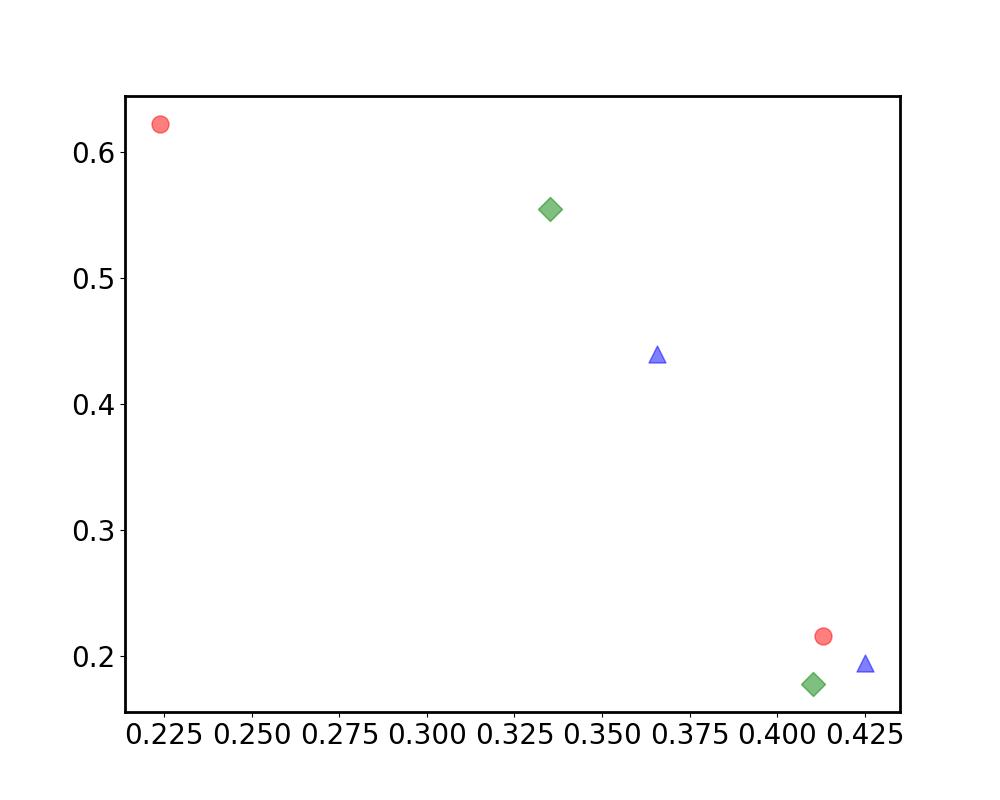
\includegraphics[width=0.4\textwidth]{figures/origin.png} 
      \label{fig:origin} %引用标签
  }
  \subfigure[属性特征向量可视化]{ %第二张子图
      \centering    %子图居中
      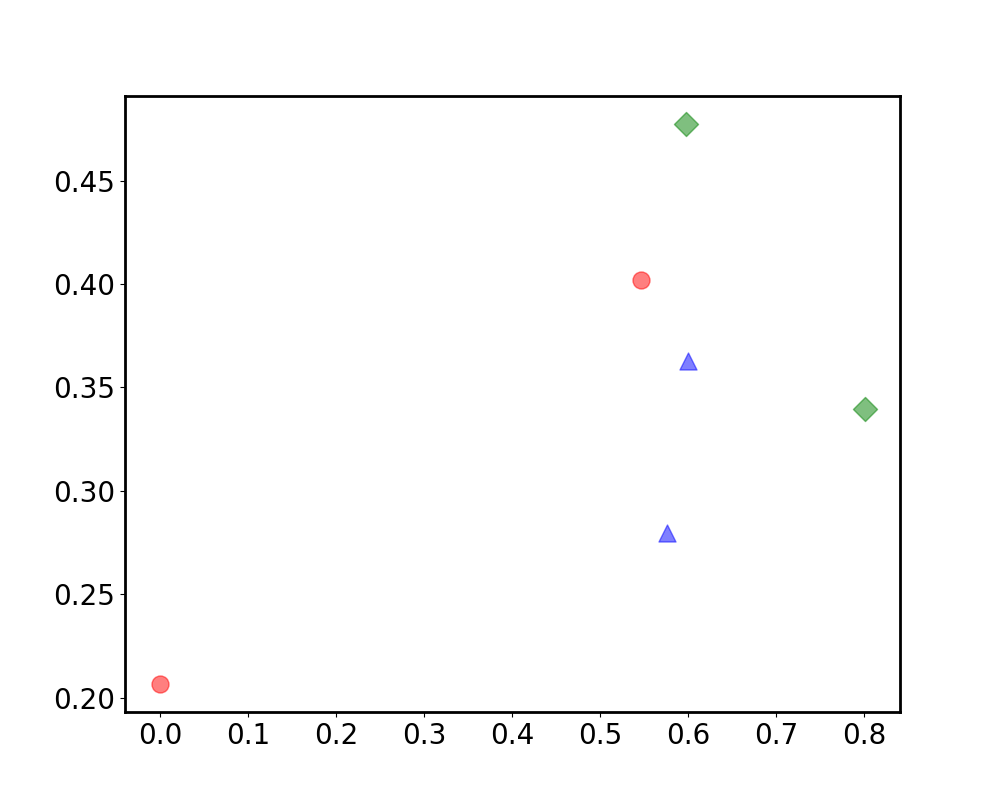
\includegraphics[width=0.4\textwidth]{figures/origin1.png}
      \label{fig:origin1} %引用标签
  }
  \caption{T-SNE技术降维后的属性特征向量可视化结果}    %大图名称
  \label{fig:originone}    %图片引用标记
\end{figure}

观察可视化结果,在\ref{fig:origin}中,向量空间的所有点是代码片段通过Word2vec初始化得到的词向量,通过简单的线性变化层将词向量转换为序列向量,然后使用t-SNE进行降维后得到的结果。在\ref{fig:origin1}中,向量空间的所有点是代码片段通过Token表征学习后得到的属性特征向量可视化结果。对比可以看到真克隆对在经过Token表征模型训练后更接近彼此,这说明,本文提出的基于预训练辅助模型的Token表征学习方法生成的真克隆对样本向量表示更相似,即可以更有效地学习代码片段Token维度的信息,生成更能代表代码片段的属性表征。

\section{本章小结}
\label{sec:Summary3}
本章主要对RLCCD中基于预训练辅助模型的Token表征学习方法的设计与实现进行详细阐述。首先介绍了Token维度的研究动机,其次介绍了Token表征学习的方法设计,具体论述了其整体框架、预训练辅助模型、表征学习,接着开展实验验证,结果表明了此方法的有效性和模型的准确性。
